\chapter{Michel decay}
~~~~~Michel decay is the most dominated decay mode of muon.
It can be calculated by Fermi theory, and the muon decay rate can be written as
\begin{equation}
 \Gamma (\mu^- \rightarrow e^- \bar \nu_e \nu_\mu) = \frac{1}{\tau_\mu} = \frac{G_F^{(e)} G_F^{(\mu)} m_\mu^5}{192 \pi^3}
\end{equation}
where the weak couplings to the electron and muon are $G_F^{(e)}$ and $G_F^{(\mu)}$, respectively.
The weak coupling is measured by experiment and can be concluded that $G_F^{(e)} = G_F^{(\mu)} = G_F^{(\tau)} = 1.16638\times10^{-5} GeV^{-2}$. 
The muon differential deacay rate is given by~\cite{kuno}
\begin{eqnarray*}
 \frac{d^2 \Gamma (\mu^-\rightarrow e^-\nu\bar\nu)}{dx \cdot d(cos\theta_e)} = &&\frac{m_\mu}{4\pi^3} W^4_{e\mu}G^2_F\sqrt{x^2-x^2_0} \\
 &\times&[F_{IS}(x)-P_\mu cos\theta_e F_{AS}(x)] \\
 &\times&[1 + \vec{P}_e(x, \theta_e) \cdot \hat{\zeta}]
\end{eqnarray*}
where $W_{e\mu} = (m_\mu^2+m_e^2)/2m_\mu$, $x = E_e/W_{e\mu}$ and $x_0 = m_e/W_{e\mu}$, respectively.
$\theta_e$ is the angle between the muon polarization $\vec{P}_\mu$ and the electron momentum $e^-$.
$\hat{\zeta}$ is the directional vector of the measurement of electron spin polarization.
The function $F_{IS}(x)$ and $F_{AS}(x)$ are the isotropic and anisotropic parts of the electron spectrum, which can be written as
\begin{gather}
 F_{IS}(x) = x(1-x) + \frac{2}{9}\rho(4x^2-3x-x_0^2) + \eta_0(1-x) \\
 F_{AS}(x) = \frac{1}{3}\epsilon\sqrt{x^2-x_0^2}\{1-x+\frac{2}{3}\delta [4x-3+(\sqrt{1-x_0^2}-1)]\}
\end{gather}
where $\rho$, $\eta$, $\epsilon$, $\delta$ are called Michel parameters.
In Standard model, they are $\rho = \frac{3}{4}$, $\eta = 0$, $\eta = 1$ and $\delta = \frac{3}{4}$, while, the experimental values are
\begin{equation}
 \rho = 0.7518\pm0.0026,~\eta = -0.007\pm0.013,~\delta = 0.7486\pm0.0038,~\epsilon = 1.0027\pm0.0084
\end{equation}
which the SM value is very close to the experimental value.

\chapter{cLFV in Standard Model}
~~~~~~The most popular explanation of charged lepton flavor violation in Standard model is one W boson is emitted through the neutrino oscillation~\cite{t2k} of $\nu_\mu \rightarrow \nu_e$.
Feynman diagram of $\mu^- \rightarrow e^-\gamma$ is shown in figure~\ref{muefy}.
\begin{figure}[H]
 \centering
 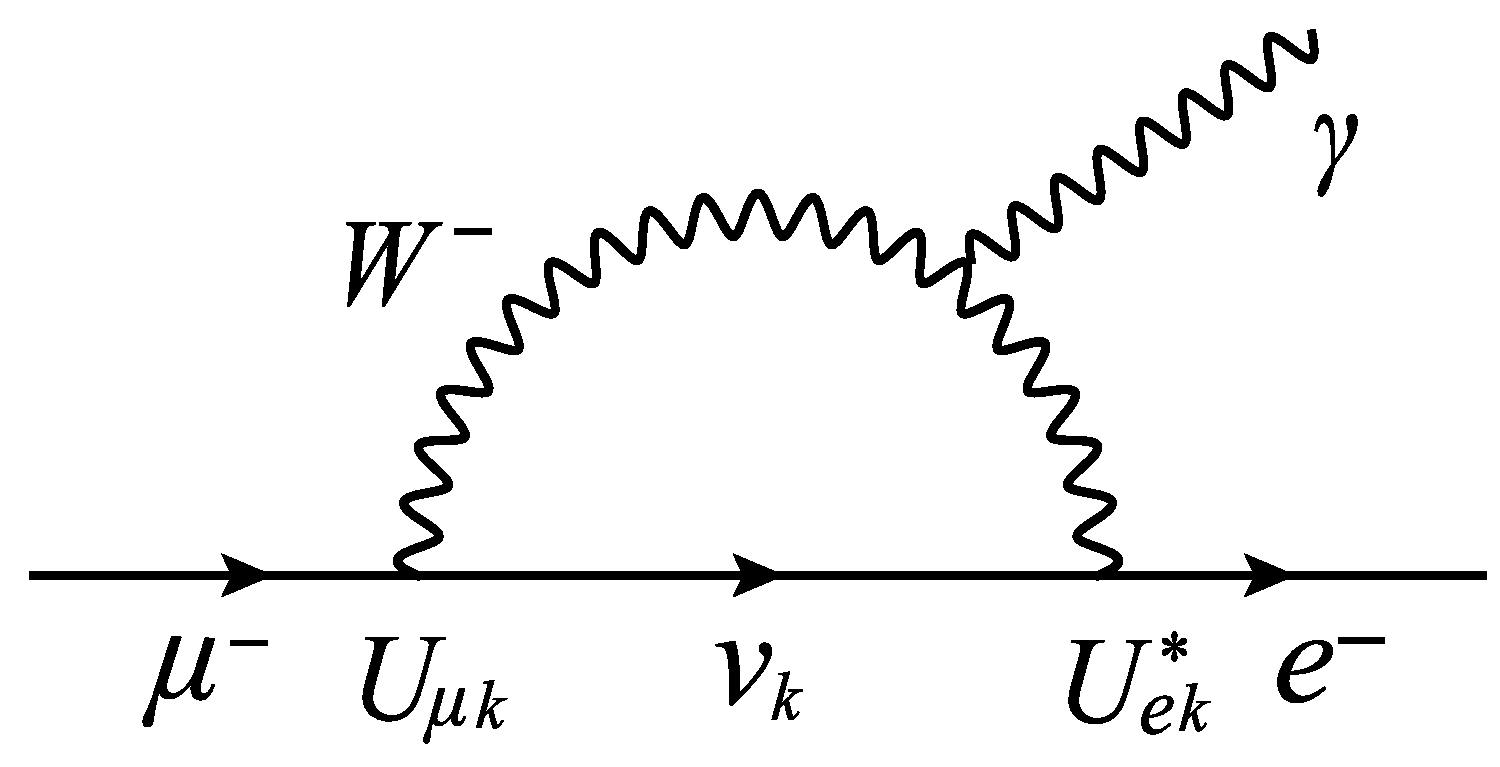
\includegraphics[scale=0.27]{chapter1/fig/SMmue.pdf}
 \caption{Feynman diagram of $\mu^- \rightarrow e^-\gamma$ predicted by massive neutrino. cLFV occurs through a neutrino oscillation, and $\gamma$ is emitted from a $W^-$}
 \label{muefy}
\end{figure}
The treatment of neutrino oscillation for three flavors is developed by 3$\times$3 PMNS matrix with mixing angle, which is written as
\begin{equation}
 \begin{pmatrix}
  \nu_e \\
  \nu_\mu \\
  \nu_\tau
 \end{pmatrix} = \begin{pmatrix}
  U_{e1} & U_{e2} & U_{e3} \\
  U_{\mu1} & U_{\mu2} & U_{\mu3} \\
  U_{\tau1} & U_{\tau2} & U_{\tau3}
 \end{pmatrix} \begin{pmatrix}
  \nu_1 \\
  \nu_2 \\
  \nu_3
 \end{pmatrix}
\end{equation}
To solve the neutrino oscillation, we start from the time evolution of the wave function, which is determined by the time evolution of the mass eigenstates and can be written as
\begin{equation}
 \mid\psi(\mathbf{x}, t)\rangle = U_{\mu1}^* \mid\nu_1\rangle e^{-i\phi_1} + U_{\mu2}^* \mid\nu_2\rangle e^{-i\phi_2} + U_{\mu3}^* \mid\nu_3\rangle e^{-i\phi_3}
\end{equation}
using the PMNS matrix, the probability of $\nu_\mu \rightarrow \nu_e$ can be described as
\begin{equation}
 P(\nu_\mu \rightarrow \nu_e) = \mid\langle\nu_e\mid\psi(\mathbf{x},t)\rangle\mid^2 = \mid-4\sum_{k=1,2,3}U_{ek}U^*_{\mu k}sin^2(\bigtriangleup_{ji})\mid^2
\end{equation}
where $\bigtriangleup_{ji} = (\phi_j-\phi_i)/2 = (m_j^2-m_i^2)\cdot L/4E_\nu$.
$L$ is the neutrino oscillation occurring distance and $(m_j^2-m_i^2)$ is the difference between the square of neutrino mass.
Thus, the decay rate of $\nu_\mu \rightarrow \nu_e$ is fixed by involving the neutrino oscillation and given by
\begin{eqnarray}
 \Gamma(\mu^- \rightarrow e^- + \gamma) &=& \frac{G_F^2 m_\mu^5}{192\pi^3}\frac{\alpha}{2\pi} P(\nu_\mu \rightarrow \nu_e) \nonumber \\
 &\simeq& \frac{G_F^2 m_\mu^5}{192\pi^3}\frac{\alpha}{2\pi}\mid U_{e3}U_{\mu3}^*\frac{\bigtriangleup m^2}{m_W^2}\mid^2
\end{eqnarray}
where $\alpha$, m$_W$ is the fine structure constant and the mass of W boson.
The ratio of the partial width $\Gamma(\mu^- \rightarrow e^-\gamma)$ to the Michel decay rate gives the branching ratio
\begin{equation}
 Br(\mu^- \rightarrow e^- \gamma) = \frac{\Gamma(\mu^- \rightarrow e^- + \gamma)}{\Gamma (\mu^- \rightarrow e^- \bar v_e v_\mu)} = \frac{\alpha}{2\pi}\mid U_{e3}U^*_{\mu3}\frac{\bigtriangleup m^2}{m_W^2}\mid^2 \textless 10^{-54}
\end{equation}

\chapter{cLFV in supersymmetry}
~~~~~~Supersymmetry (SUSY) is the most possible candidate in the physics beyond the Standard model, which can explain the hierarchy problem and Higgs' mass perfectly.
It is a proposed extension of SM by including the superpartner for each particle.
For instance, each ferimon has its superpartner, boson, and vice versa.
In the prediction of SUSY model which shown in figure~\ref{susyfy}, the cLFV is occurred by the slepton mixing.
\begin{figure}[H]
 \centering
 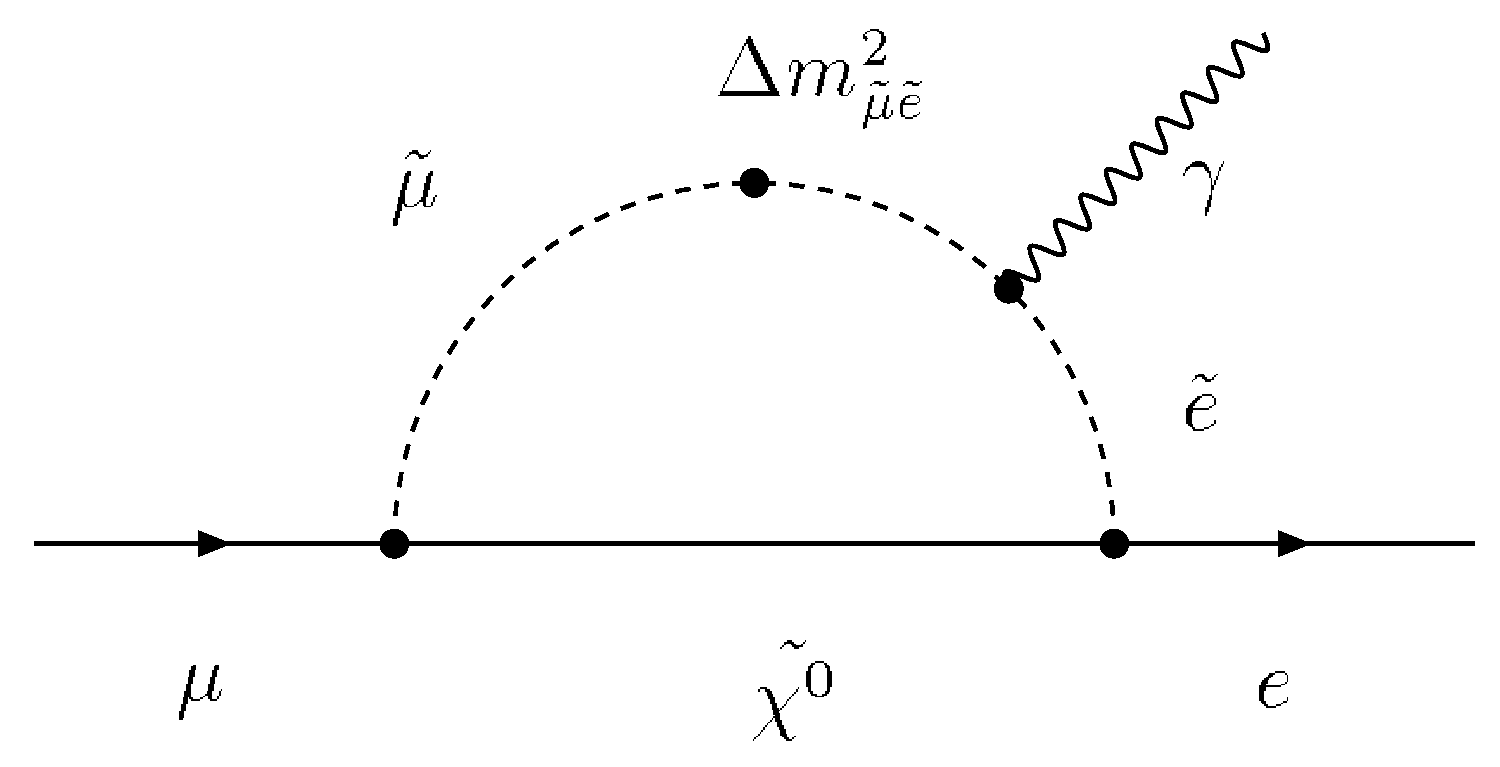
\includegraphics[scale=0.3]{chapter1/fig/SUSYmue.pdf}
 \caption{Feynman diagram of $\mu^- \rightarrow e^-\gamma$ predicted by slepton mixing. it occurs through its superpartner $\tilde{\mu}$ and $\tilde{e}$ mixing.}
 \label{susyfy}
\end{figure}
The branching ratio of $\mu \rightarrow e\gamma$ is given similarly to the SM by~\cite{kuno2}
\begin{equation}
 Br(\mu \rightarrow e\gamma) = \frac{\alpha}{2\pi}\mid\sum_{k}\tilde{U}_{ek}\tilde{U}^*_{\mu k}\frac{\Delta m_k^2}{m_S^2}\mid^2(\frac{m_W}{m_S})^4
\end{equation}
where $m_S$ is the typical scale of scalar masses, $\tilde{U}$ is the mixing matrix between sleptons and leptons, and $\Delta m_k^2$ is the square of mass difference between the kth and 1st sleptons.

From figure~\ref{susyfy}, the mixing $\Delta m_{\tilde{e}\tilde{\mu}}^2$ between a smuon $\tilde{\mu}$ and a selectron $\tilde{e}$ plays a key role in cLFV.
This slepton mixing parameter, $\Delta m_{\tilde{e}\tilde{\mu}}^2$ is given by the slepton mass matrix $m_{\tilde{l}}^2$
\begin{equation}
 (m_{\tilde{l}}^2)_{ij} = (m_lm_l^{\dagger})_{ij} + (\tilde{m}_l^2)_{ij} = 
 \begin{pmatrix}
  m_{\tilde{e}\tilde{e}}^2 & \Delta m_{\tilde{e}\tilde{\mu}}^2 & \Delta m_{\tilde{e}\tilde{\tau}}^2 \\
  \Delta m_{\tilde{\mu}\tilde{e}}^2 & m_{\tilde{\mu}\tilde{\mu}}^2 & \Delta m_{\tilde{\mu}\tilde{\tau}}^2 \\
  \Delta m_{\tilde{\tau}\tilde{e}}^2 & \Delta m_{\tilde{\tau}\tilde{\mu}}^2 & m_{\tilde{\tau}\tilde{\tau}}^2
 \end{pmatrix}
\end{equation}
where $(m_lm_l^{\dagger})_{ij}$ is the lepton mass matrix and $(\tilde{m}_l^2)_{ij}$ is the term of SUSY breaking, respectively.
As the scenario of SUSY, SUSY-GUT and SUSY-Seasaw contribute to the off-diagonal terms.

\subsubsection{SUSY-GUT}
~~~~~Supersymmetric grand unified theories (SUSY-GUT) is the extension of grand unified theories with supersymmetry.
Three gauge coupling constants of electromagnetic, weak and strong interaction are unified to SU(5) coupling constant at scale of 10$^6$ GeV, which is also called GUT scale.
Due to the generation of the off-diagonal elements in slepton mass matrix, the cLFV is occurred with big branching ratio.
$\Delta m_{\tilde{\mu}\tilde{e}}^2$ is given by
\begin{equation}
 \Delta m_{\tilde{\mu}\tilde{e}}^2 \propto \frac{3m_0^2 + A_0^2}{8\pi^2}h_t^2V_{td}^*V_{ts}ln\frac{M_{GUT}}{M_{R_3}}
\end{equation}
where $m_0$ and $A_0$ are the universal scalar mass and the universal trilinear coupling respectively.
$V_{td}$ and $V_{ts}$ are the elements in the CKM matrix.
$M_{R_3}$ is the mass of the right-hand neutrino.
$M_{GUT}$ is the GUT scale ($\approx$ 2$\times$10$^{18}$ GeV).
and $h_t$ is the Yukawa coupling constant of top quark.
Figure~\ref{susygut} shows the prediction of the branching ratio of $\mu \rightarrow e$ conversion with Ti target in SUSY-GUT model~\cite{kuno}, which is higher than the prediction of SM with the order of 10$40$.
Here, $m_{\tilde{e}_R}$ is the mass of right-hand electron, and $\mu$ is the parameter defined by Higgs and Higgsino.
\begin{figure}[H]
 \centering
 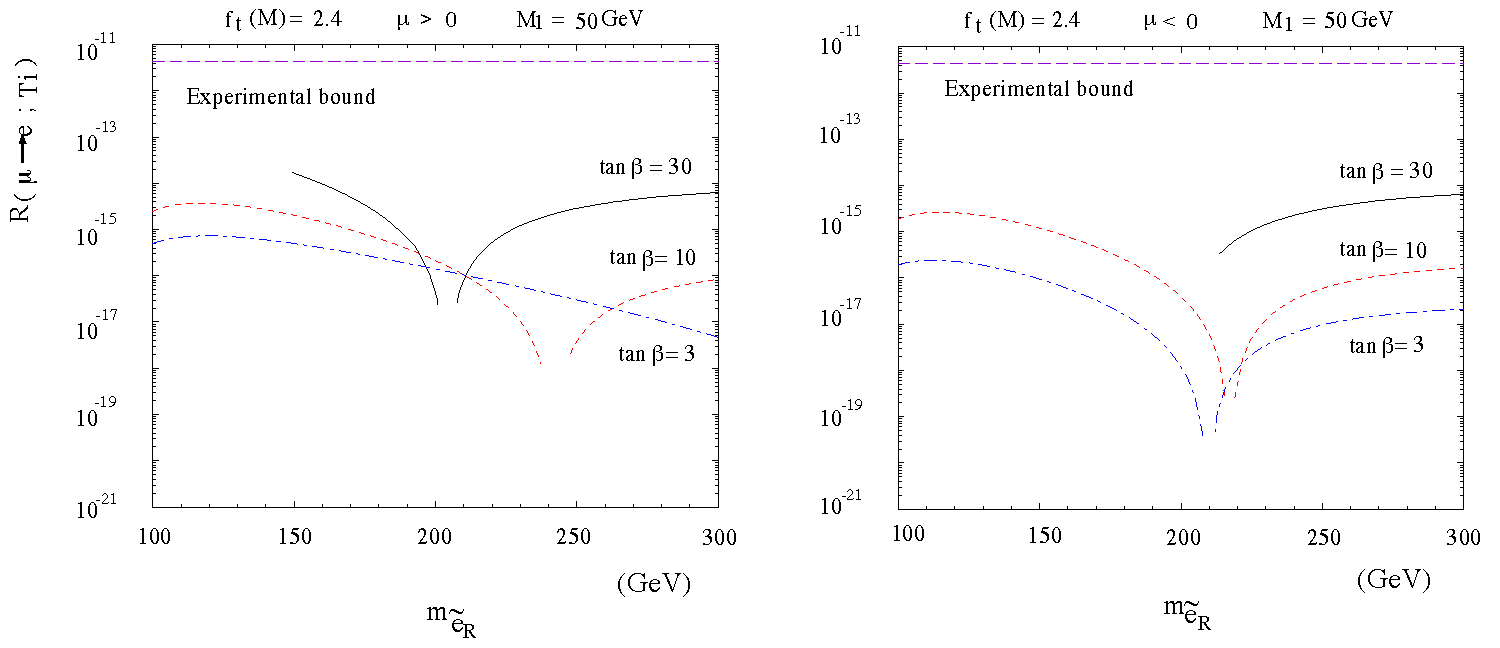
\includegraphics[scale=0.68]{chapter1/fig/gut.pdf}
 \caption{Pridiction of branching ratio of $\mu \rightarrow e$ conversion in SUSY-GUT SU(5). Mass of right-hand $\tilde{e}$ can be observed indirectly if the $\mu \rightarrow e$ conversion experiment gets more precision sensitivity.}
 \label{susygut}
\end{figure}

\subsubsection{SUSY-Seasaw}
~~~~~SUSY-Seasaw model is another scenario for the prediction of cLFV by including the right-hand neutrino.
From the right-hand neutrino mass term, the slepton mixing can be obtained as well.
The slepton mixing between muon and electron depends on the solar neutrino oscillation and atomspheric neutrino oscillation~\cite{hisano}.
Thus, $\Delta m_{\tilde{\mu}\tilde{e}}^2$ can be written as
\begin{equation}
 \Delta m_{\tilde{\mu}\tilde{e}}^2 \propto \frac{3m_0^2+A_0^2}{8\pi}h_\tau^2U_{\tau e}^*U_{\tau\mu}ln\frac{M_{GUT}}{M_{R_3}}
\end{equation}
where $U_{\tau e}^*$ and $U_{\tau\mu}$ are the elements of PMNS matrix.
$h_\tau$ is the Yukawa coupling constant of $\tau$.
The prediction of branching ratio of $\mu \rightarrow e\gamma$ by SUSY-Seasaw is given in figure~\ref{susyseasaw}.
Similar to the prediction of SUSY-GUT model, it also predicts the higher branching ratio for cLFV.
\begin{figure}[H]
 \centering
 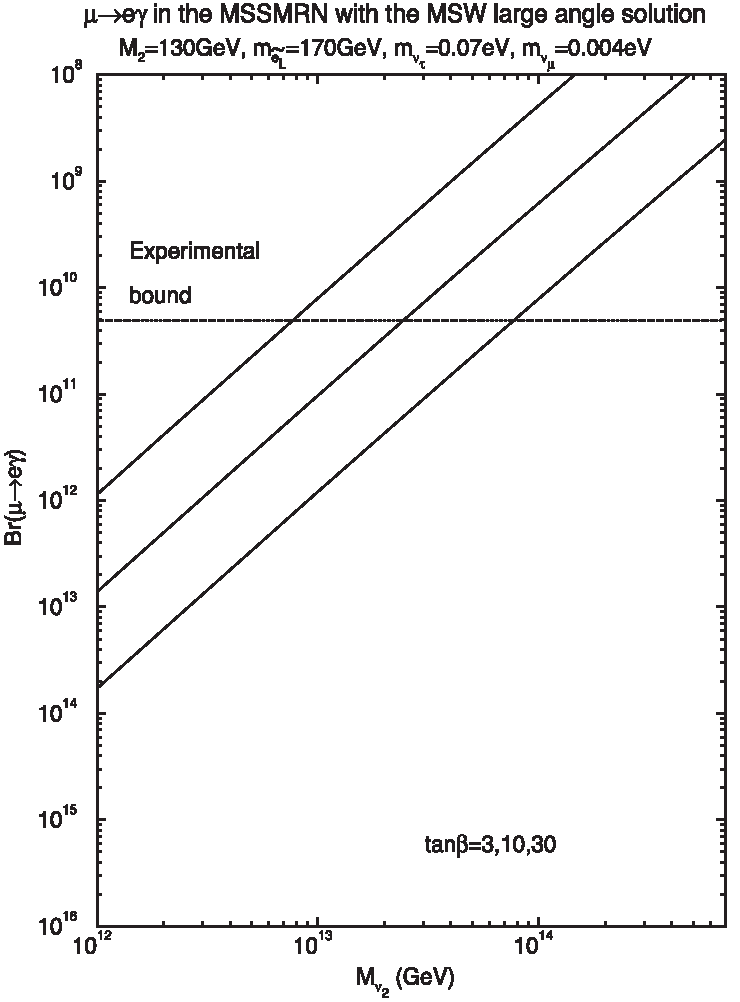
\includegraphics[scale=0.6]{chapter1/fig/susyseasaw.pdf}
 \caption{Prediction of branching ratio of $\mu \rightarrow e\gamma$ in SUSY-Seasaw model.}
 \label{susyseasaw}
\end{figure}

\chapter{Impact of cLFV}
~~~~~Because of the higher branching ratio predicted by BSM, in addition, the branching ratio depends on the experimental sensitivity, the discovery of cLFV plays an important role in seeking for the BSM.
In W. Altmannshofer's paper, the sensitivities of several flavor observables to a variety of BSM models are listed in figure~\ref{predict}.
\begin{figure}[H]
 \centering
 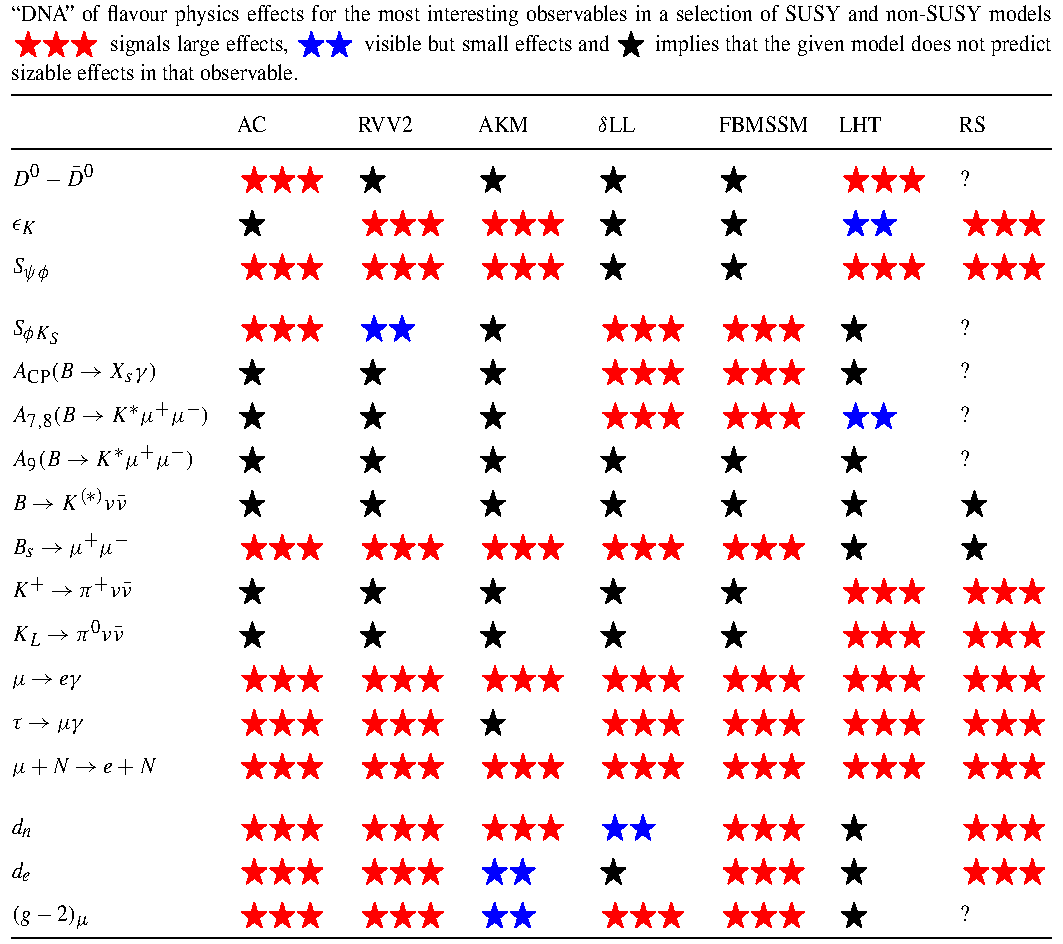
\includegraphics[scale=0.7]{chapter1/fig/predict.pdf}
 \caption{\it The size of the observable flavor effect for a variety of SUSY and non-SUSY models.}
 \label{predict}
\end{figure}
where AC, RVV2, AKM, $\delta$LL, FBMSSM, LHT and RS are Abelian U(1) flavor symmetry model, non-Abelian model, Antush-King-Malinsky SU(3) flavor symmetry model, flavor models with pure CKM-like left handed currents, flavor-blind MSSM, littles Higgs with T-parity and Randll-Sundrum model~\cite{wolf}.
In all these decay modes, $\mu \rightarrow e$ coversion and $\mu \rightarrow e\gamma$ contributes a large effect on every theory, which means the BSM is easy to be found in these two modes with high probability.

\chapter{Magnetic field interpolation}
~~~~~Suppose there is field map, it only gives us the coordinate (x, y, z), magnetic field vector (B$_x$, B$_y$, B$_z$) and magnetic field (B), so we have many points with magnetic field.
If the particle goes through this point, the magnetic field is already there.
However, the magnetic field has to be interpolated when the particle goes through the point we haven't.
The simple way to interpolate the field is to weight the field in a box.

There is box which vertices are the known coordinate of field map.
Each vertices can be written as
\begin{eqnarray}
 \vec{r_1} = (x_{lt}, y_{lt}, z_{lt}) \nonumber \\
 \vec{r_2} = (x_{gt}, y_{lt}, z_{lt}) \nonumber \\
 \vec{r_3} = (x_{gt}, y_{gt}, z_{lt}) \nonumber \\
 \vec{r_4} = (x_{gt}, y_{gt}, z_{gt}) \nonumber \\
 \vec{r_5} = (x_{lt}, y_{gt}, z_{lt}) \nonumber \\
 \vec{r_6} = (x_{lt}, y_{gt}, z_{gt}) \nonumber \\
 \vec{r_7} = (x_{lt}, y_{lt}, z_{gt}) \nonumber \\
 \vec{r_8} = (x_{gt}, y_{lt}, z_{gt})
\end{eqnarray}

where the x$_{gt}$ is the greater value and x$_{lt}$ is the less value along the x direction.
Thus, the weight of x, y and z axis in this box can be written as
\begin{equation}
 t = \frac{x_0-x_{lt}}{x_{gt}-x_{lt}}, ~~~~~~~u = \frac{y_0-y_{lt}}{y_{gt}-y_{lt}}, ~~~~~~v = \frac{z_0-z_{lt}}{z_{gt}-z_{lt}}
\end{equation}

where (x$_0$, y$_0$, z$_0$) is the position of the particle and (t, u, v) is the weight on this position.
(x$_0$, y$_0$, z$_0$) must be inside this box.
Therefore, the magnetic field of this position is
\begin{eqnarray}
 B_i(\vec{r_0}) = &&(1-t)(1-u)(1-v) B_i(\vec{r_1})   \nonumber \\
 				  &+& (1-u)(1-v)t B_i(\vec{r_2})	 \nonumber \\
				  &+& tu(1-v) B_i(\vec{r_3})		 \nonumber \\
				  &+& tuv B_i(\vec{r_4})			 \nonumber \\
				  &+& (1-t)u(1-v) B_i(\vec{r_5})	 \nonumber \\
				  &+& (1-t)uv B_i(\vec{r_6})		 \nonumber \\
				  &+& (1-t)(1-u)v B_i(\vec{r_7})	 \nonumber \\
				  &+& t(1-u)v B_i(\vec{r_8})				   \\
&& (x_{lt} \le x_0 \le x_{gt}, y_{lt} \le y_0 \le y_{gt}, z_{lt} \le z_0 \le z_{gt})	  \nonumber 
\end{eqnarray}
